
\section{血压估计方法}
\label{sec:techniques}

\subsection{方法框架与演进}
\label{sec:evolution}

PPG估计血压模型需要考虑四个问题：输入用什么表征、采用什么模型、监督信号从哪里来、是否使用受试者的个性化数据。可以把现有工作划为三条路线，\cref{fig:routes}(a) 中使用不同的颜色表示不同的路线：手工特征配合浅层回归的传统机器学习路线（蓝）、端到端深度学习路线（紫），以及先大规模预训练再微调的路线（橙）。三条路线都可以实现血压估计，差别主要在监督来源与部署成本：传统路线依赖于手动特征与血压标签；端到端路线通过深度学习网络学习表征，但需要更多带标签数据；预训练路线先在大量的无标注PPG上学习通用表征，再用少量标签完成下游微调。

\begin{figure*}[t]
\centering
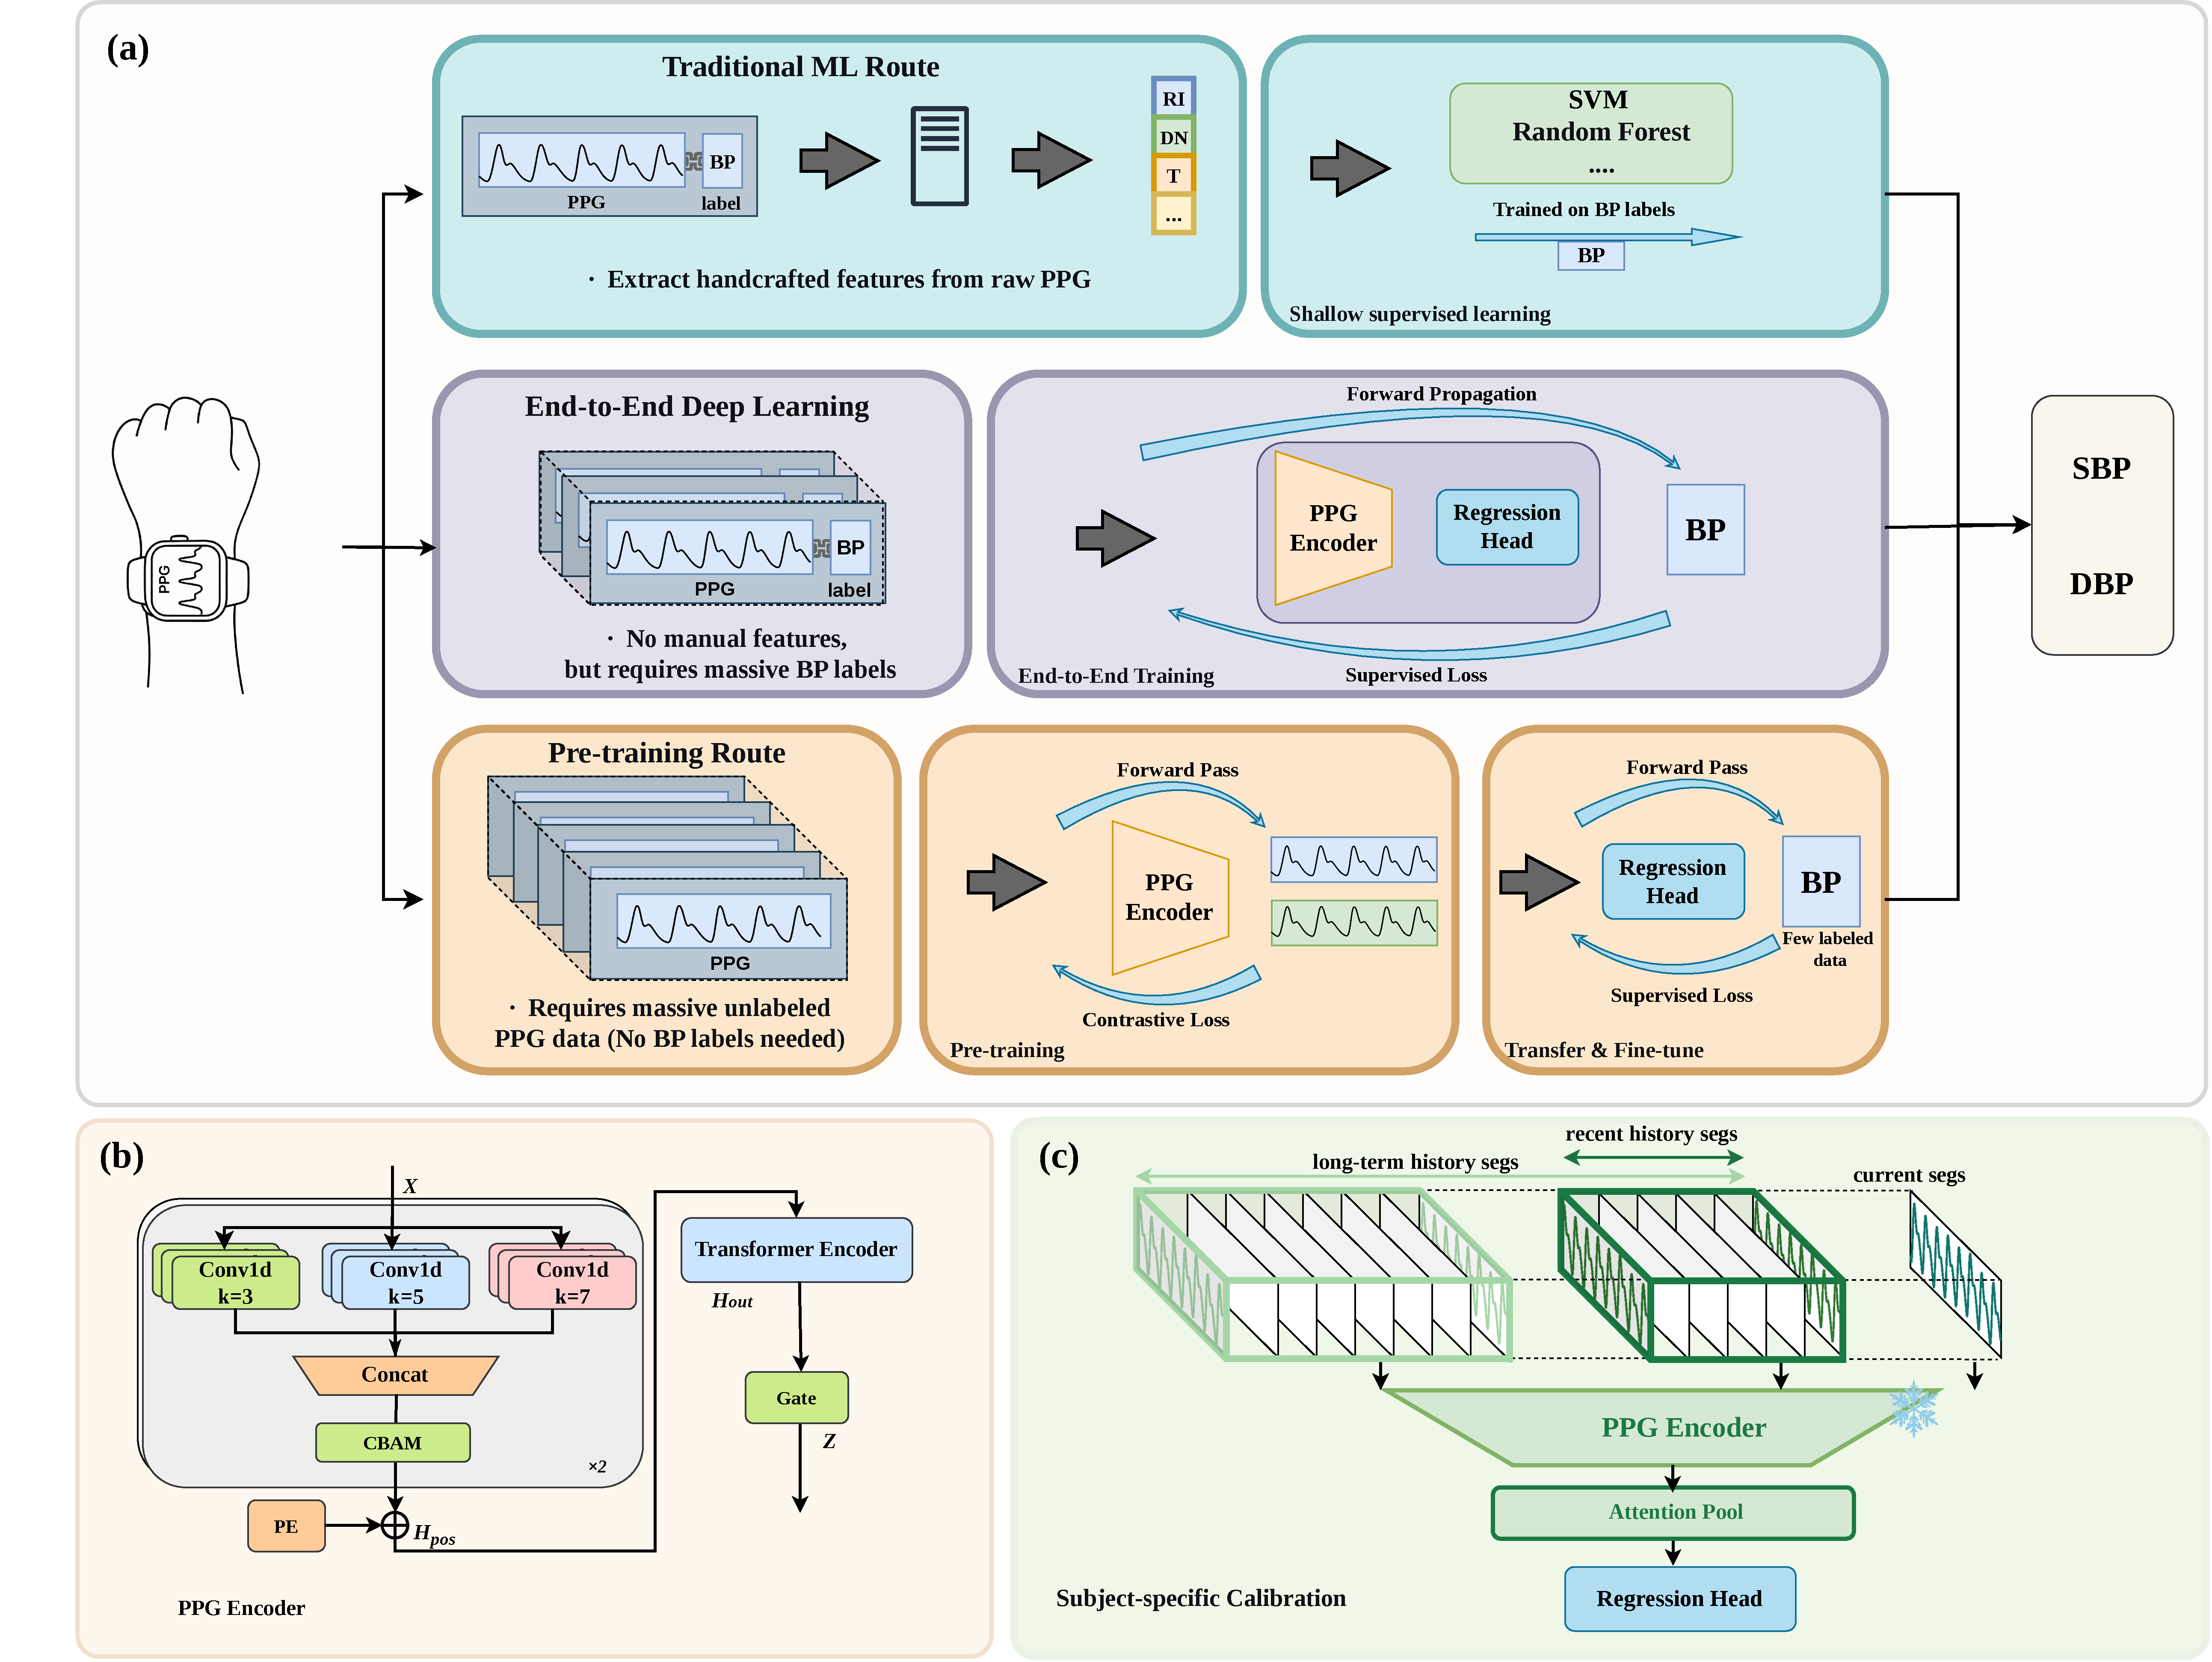
\includegraphics[width=\textwidth]{4_血压估计方法/figs/三路线图.drawio.pdf}
\caption{由 PPG 估计血压的方法框架。(a) 三条技术路线：传统机器学习（蓝）、端到端深度网络（紫）与预训练—微调（橙），三者在输入表征、监督信号与校准数据上各有取舍；(b) PPG编码器（SIFPBPNet）：原始波形及其一、二阶导数构成三通道输入，经多尺度一维卷积、CBAM 注意力、位置编码与 Transformer 编码器得到片段表征；(c) 个体化校准：长期与近期历史片段经冻结的编码器与注意力池化聚合成稳态表征，与当前片段融合后回归个体血压。}
\label{fig:routes}
\end{figure*}

手工特征路线以\cref{sec:physio}讨论的形态、频域与导数域特征为输入，配合支持向量机、随机森林或多线性回归估计血压\cite{haddad2022continuous,cisnal2024robust}。其特征有明确的生理含义，模型可解释、训练代价低，在连续监测中应用较广；但特征依赖先验，对运动伪影与佩戴松紧敏感，换数据集常需重做特征筛选，跨库迁移时性能衰减明显。这一局限把研究推向端到端学习。

三条路线共同的难点是个体差异：同一段波形在不同受试者身上可能对应不同血压水平，人群模型倾向于向均值回归。\cref{fig:routes}(c) 所示的个体化校准则为缓解这一问题而引入，后文\cref{sec:calib}展开。

\subsection{端到端深度网络与 PPG 编码器}
\label{sec:deep}

端到端路线让网络直接从原始波形或时频表示回归血压。CNN是较早的用于回归血压的深度学习模型\cite{liu2019cuffless}，此后循环网络与Transformer相继引入：卷积擅长局部形态，循环结构建模逐拍依赖，注意力机制便于融合多通道信息，三者常被组合使用。在这一路线中编码器的设计十分关键，\cref{fig:routes}(b) 为SIPFBP的PPG编码器结构：输入为原始 PPG 及其一阶、二阶导数构成的三通道信号；三路并行的一维卷积分别取 $k=3,5,7$ 的感受野，提取不同时间尺度的局部形态；拼接后经 CBAM 的通道与空间注意力抑制噪声、突出与血压相关的区域；再叠加位置编码保留片段的绝对时序，送入Transformer实现的长程表征提取；最后经全局池化与门控得到片段表征。

\cref{fig:routes}(b)的结构展现了目前编码器的共同取向：多尺度卷积负责局部形态，注意力负责特征选择与时序建模，表征由数据驱动。代价是需要大量有标签的样本，且中间表征难以对应到具体的生理解释，可解释性弱。一个合适的编码器既可以使用端到端的方式训练，也可以用无监督预训练的方式进行训练。

\subsection{大规模预训练}
\label{sec:pretrain}

预训练路线对应\cref{fig:routes}(a) 的橙色分支：先在海量无标注片段上预训练编码器，再用少量标注数据微调下游回归头。掩码重建与对比学习为此提供了成熟范式\cite{he2022mae,chen2020simclr}；PaPaGei 与 AnyPPG 将这一范式带到 PPG，借助大规模记录学习通用表征\cite{pillai2025papagei,nie2025anyppg}。近期的改进集中在掩码粒度与先验引入：HiMAE 用分层掩码同时保留粗、细两种时间尺度\cite{lee2026himae}，另有工作按小波分解的多尺度结构组织掩码单元、以外周参考信号引导跨模态重建\cite{thukral2026wavelet,zhou2026physiology}。另一个方向是让掩码单元与生理节律对齐：以完整心动周期作为掩码的基本单元，并借助受试者的纵向历史片段提供个体上下文，可避免跨心搏掩码造成的语义混杂。

预训练的价值在于缓解血压标签稀缺：无标注 PPG 易于大规模采集，而同步袖带标签昂贵且稀疏。其局限是预训练目标与血压回归之间存在语义差距，微调阶段仍需一定数量的标签，且不同预训练语料带来的增益在跨设备场景下并不稳定。

\subsection{个体化校准与多模态融合}
\label{sec:calib}

预训练解决通用表征，个体差异仍需在部署端处理。常见做法分三档：一次袖带测量做单点校准、按时段重复校准，或用元学习与少样本微调快速适配新受试者；仅用数分钟个体数据训练混合推理模型，可把免频繁校准的可用期延长到月级\cite{mekonnen2024accurate}。

\cref{fig:routes}(c) 给出一种更系统的校准思路：不直接把当前片段映射到血压，而是先从用户的历史片段中挖掘个体稳态信息。具体而言，长期与近期的历史片段与当前片段经冻结的 PPG 编码器得到表征；历史片段的表征以注意力池化聚合为稳态表征，刻画该用户的血压基线与波动模式；稳态表征再与当前片段表征融合，经回归头输出个体化血压。SIFPBPNet 以图注意力网络聚合数量可变的历史片段，并用年龄回归、高血压判别与血压变异性检测等辅助任务预训练该路径，使稳态表征携带与血压相关的个体先验，两阶段训练中历史数据与评估数据按受试者隔离\cite{tang2026sifpbpnet}。该模块可即插即用地接入不同骨干网络，在多个骨干上带来收缩压 MAE 2.8\%--13.1\% 的相对降低。

另外就是多模态融合：在 PPG 之外引入毫米波脉搏波、心电或加速度计，补充压力波形与运动信息\cite{zheng2024bp3,mieloszyk2022comparison}。校准与融合的共同代价是部署复杂度：前者需要历史数据与隐私保护，后者需要额外传感器与同步采集。

\subsection{小结}
\label{sec:techniques_summary}

血压估计的方法的重心已从设计特征移到学习表征，再移到学表征并校准个体。\cref{fig:routes} 的三部分恰好对应此变化过程：\cref{fig:routes}(a)：路线选择决定监督来源，\cref{fig:routes}(b)：编码器设计决定表征质量，\cref{fig:routes}(c)：个体化校准决定部署后的精度保持。模型容量与预训练规模仍在快速提升，但跨数据集、跨设备的性能衰减尚未根本解决；能否在有限校准数据下保持鲁棒，仍是区分方法优劣的关键。